\chapter{The Stern-Gerlach Experiment}

\section{Spin Angular Momentum}

Let's start with a system that is pretty much as far away from the quantum world as possible -- the Earth and Sun, as shown in Figure \ref{fig_sun_earth}.  With its total motion, the Earth has two kinds of angular momentum:  \emph{orbital} angular momentum $\vec{L}$ from its orbit around the sun, and \emph{spin} angular momentum $\vec{S}$, resulting from its 24 hour rotation.  Of course, the spin angular momentum in this case is due to adding up the orbital angular momentum $\vec{L}_i = \vec{r}_i \times \vec{p}_i$ of each of the tiny pieces of the Earth, but we'll keep the distinction because this is definitively not the case in quantum systems as we'll see.  Note that the two kinds of angular momentum for the Earth point in different directions since the rotation axis of the Earth is tilted 23$^\circ$ from the orbital plane.

\begin{figure}
\centering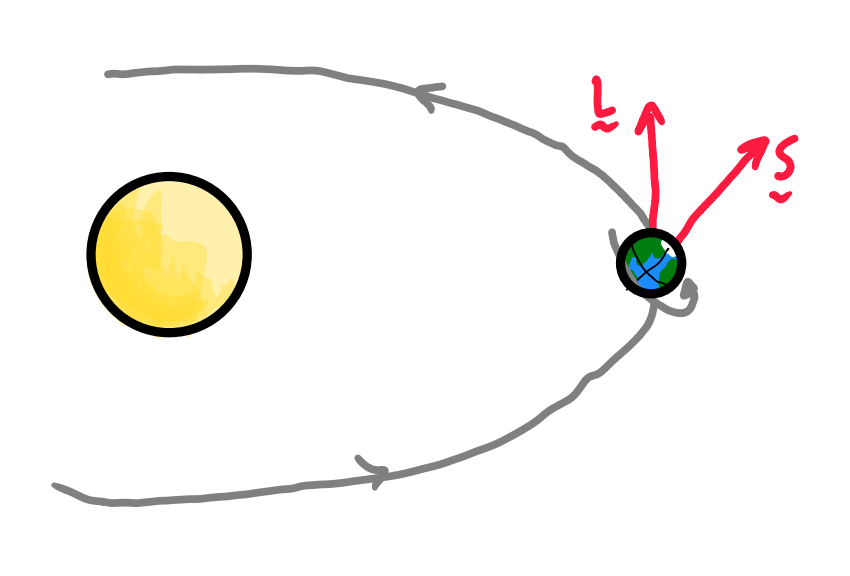
\includegraphics[width=0.5\linewidth]{Figures/Chapter 1/fig_sun_earth.png}
\caption{The Earth goes around the Sun every 365 days (orbital angular momentum) and rotates around its axis every 24 hours (spin angular momentum).}
\label{fig_sun_earth}
\end{figure}

As a simple quantum system, consider an electron in orbit around a proton -- a hydrogen atom.  The electron has orbital angular momentum just like the Earth (depending on what state it's in), and it also has spin angular momentum.  Careful, though, as the electron doesn't rotate like the Earth -- how can it when it has essentially no size or diameter to spin?  Despite this, it has measurable intrinsic angular momentum, which we'll call \emph{spin} $\vec{S}$.  Since spin is a vector, it has components $(S_x, S_y, S_z)$, and thus to specific the spin of the electron we use three different numbers; keep this in mind for later.

Suppose we put a stationary electron in a magnetic field $\vec{B}$.  Since the electron is stationary, the Lorentz force
\[
\vec{F} = q\vec{v} \times \vec{B}
\]
is zero.  But the electron's spin angular momentum gives it a magnetic dipole moment $\vec{\mu}$, and it's then possible for an \emph{inhomogeneous} magnetic field to exert a force (see Griffiths \emph{Introduction to Electrodynamics}, fourth edition, section 6.2)
\begin{equation}
\vec{F} = \grad (\vec{\mu} \cdot \vec{B}).
\end{equation}



%
%
%

\section{The Stern-Gerlach Experiment}

The 

%
%
%

\section{Extending the Experiments}

The 

%
%
%



\section*{Problems}
\addcontentsline{toc}{section}{Problems}
\markright{Problems}%

\begin{problem}[Electron spin]
How fast would the surface of an electron be going if it had ....
\end{problem}

